\documentclass[a4paper,twocolumn,openany,nodeprecatedcode, justified]{dndbook}
\pdfpagewidth=\paperwidth
\pdfpageheight=\paperheight

\usepackage[english, greek, main=czech]{babel}

\usepackage[utf8]{inputenc}
\usepackage[T1]{fontenc}
\usepackage[singlelinecheck=false]{caption}
\usepackage{listings}
\usepackage{shortvrb}
\usepackage{stfloats}

\usepackage{titling}
\usepackage{fancyhdr}

\usepackage{gfsneohellenic}

\usepackage{graphicx}
\graphicspath{ {./images/} }
\usepackage{wrapfig}

\usepackage{hyphenat}
\hyphenation{zpro-střed-ko-vá-va-jí vo-jen-sko ad-mi-nis-tra-tiv-ních cha-rak-te-ris-ti-kách A-mau-ris-tion A-mau-ris-ti-o-nu Prin-ci-pá-tu způ-so-bem zá-zrak ji-ho-ji-ho-vý-chod-ně Prin-ci-pát or-ga-ni-zo-va-ná Ca-er-le-ons-kém}

\newcommand{\grnh}[1]{\textneohellenic{\ensuregreek{#1}}}

\usepackage{indentfirst}

\newcommand{\bi}{\begin{itemize}}
	\newcommand{\ei}{\end{itemize}}
\newcommand{\ben}{\begin{enumerate}}
	\newcommand{\een}{\end{enumerate}}

\usepackage[normalem]{ulem}

\frenchspacing


\pretitle{% add some rules
	\begin{center}
		\Huge\bfseries
	}%, make the fonts bigger, make the title (only) bold
	\posttitle{%
	\end{center}%
	\noindent\vrule height 2.5pt width \textwidth
	\vskip .75em plus .25em minus .25em% increase the vertical spacing a bit, make this particular glue stretchier
}
\preauthor{%
	\begin{center}
		\Large \lineskip 0.75em%
		\vrule height 0.4pt width .25\textwidth\par
		\begin{tabular}[t]{@{}l@{}}%
		}
		\postauthor{%
		\end{tabular}
		\vskip -.5em
		\par
		\vrule height 0.4pt width .25\textwidth\par
	\end{center}%
}
\predate{%
	\begin{center}
		\Large
	}
	\postdate{%
		\begin{figure}[b]
			\vspace{-4cm}
			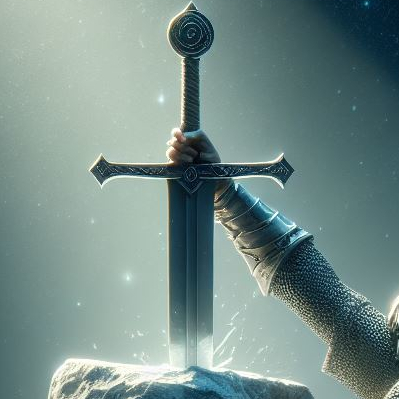
\includegraphics[width=0.4\textwidth]{SwordInStoneCross.jpg}
			\centering
		\end{figure}
	\end{center}%
}

\captionsetup[table]{labelformat=empty,font={sf,sc,bf,},skip=0pt}

\MakeShortVerb{|}

\lstset{%
	basicstyle=\ttfamily,
	language=[LaTeX]{TeX},
	breaklines=true,
}

\title{
	Cei \& Enid\\
	\LARGE Trojsvětí
}
\author{Vít Matějíček \and Barbora Šašková \and Šárka Doležalová \and Filip Kastl}
\date{\today}


\begin{document}
	\DndSetThemeColor[BrGreen]
	
	\frontmatter
	
	\maketitle
	
	\tableofcontents
	
	\mainmatter%
	
	\part{Padající ostrovy}
	\chapter{Svět}
	\section{Trojsvětí}
	\DndDropCapLine{T}{}rojsvětí je modrá prázdnota nad kterou se vznáší kusy země -- ostrovy. Každý
	ostrov je jiný. Některé jsou velké, jiné malé. Některé jsou prázdné, jiné jsou
	domovem celých civilizací. Některé jsou technologicky velice vyspělé (až sci-fi),
	některé jsou na úrovni doby kamenné.
	
	Když se dostanete na okraj ostrova, atmosféra ustoupí a vy vidíte na obzoru
	další ostrovy plující nicotou. Co je dole v propasti, nikdo neví. Proč se světu
	říká Trojsvětí a co udržuje ostrovy od toho, aby padaly možná někdo tuší, ale
	vy nikoho takového neznáte.
	
	Někteří tvrdí, že Trojsvětí kdysi tvořil souvislý povrch rozpínající se na všechny strany do nekonečna, který se teprve po nějakém magickém kataklyzmatu roštěpil na miliardy ostrůvků plujících volně prázdnotou nad lehce zářící namodralou propastí. Jiní si s~takovými hloupostmi nelámou hlavu a prostě akceptují věci, tak jak holt jsou.
	
	\section{Padající ostrovy}
	Víte, jak jsem výše psal, že ostrovy nepadají? Tak několik z nich nedávno padat
	začalo. Z dotyčných ostrovů se postupně oddělují kusy (klidně celá vesnice). Po
	tom, co kus horniny a hlíny odpadne od ostrova, odpluje od něj o několik desítek
	metrů a pak začíná pomaličku klesat dolů. Obyvatelé padajících ostrovů se k
	situaci staví různé, ale většina z nich prostě panikaří. Některé ostrovy už se
	tímto způsobem zcela rozpadly a zřítily. Těžko říct, jestli je to fenomén globální
	nebo jestli se týká jen pár sousedních ostrovů.
	
	Vy se v kampani budete po padajících ostrovech pohybovat. Očekávám, že
	většina z vás bude buď pocházet z nějakého padajícího ostrova nebo bude k
	němu mít alespoň nějakou vazbu (např. mám tam kamarády, nechci, aby jim
	spadl ostrov / rozpadl se).
	
	\section{Záporák}
	Někteří z vás se mohli setkat se záhadnou postavou v černých róbách a kápi.
	Poslední dobou se vyskytuje na ostrovech, které někdy brzo před nebo po jejím
	výskytu začaly padat. Ti z vás, kteří se snaží zjistit více o padání ostrovů, mají
	podezdření, že tato postava by s tím mohla mít něco společného. Předpokládáte,
	že je to Turista vzhledem k tomu, že se umí pohybovat po ostrovech.
	
	Je možné, že se někteří z vás snaží Záporáka polapit z ještě jiných důvodů.
	Pokud tomu tak je, domluvíme se ještě, co vám provedl, že ho teď stíháte.
	
	
	
	\section{Turisté}
	
	\DndDropCapLine{M}{}álokomu se však poštěstí mezi Ostrovy cestovat. Jen Turisté mají nástroje potřebné k~něčemu takovému. A~vy jste jedněmi z~nich. Každý z~vás pochází z~jiného ostrova, kde vás už před nějakou dobou Turisté naverbovali. Většina z~vás už cestovala i s~jinými družinami Turistů. Vaše momentální sestava za sebou má jen několik splněných úkolů, ale i to je dost na to, abyste se dostatečně seznámili a spřátelili.
	
	\subsection{Brány}
	
	Na každém ostrově se někde nachází Brána. Brány jsou portály vedoucí z~ostrova na ostrov. Když ale takovou Branou člověk projde, nelze dobře určit, kde skončí. Jejich aktivace je navíc pokaždé jiný, často bizardní a náročný proces. Jak při ní postupovat lze jen hádat. Není to nemožné, ale nestává se často, že by se někomu záměrně bránu podařilo aktivovat bez Turistického náčiní. To už se spíš brána náhodně aktivuje sama (a pravděpodobně v~tu nejhorší chvíli).
	
	\subsection{Úkoly}
	
	Turistická organizace je řízena záhadným způsobem. Turistická družina s~sebou typicky nese příkazy pro mnoho jiných družin s~tím, že ví, komu je mají předat, ale netuší, kdy se s~dotyčným setkají. Kromě toho samozřejmě plní úkoly a následují cesty, podle svých vlastních rozkazů. To zahrnuje prozkoumávání neprozkoumaného, verbování nových členů a mnoho dalšího. Zadání však bývá tak vágní, jak jen to jde, a už jen dostat se tam, kde máte být, může být obtížnější než samotný úkol.
	
	\section{Cestovní výbava Turisty}
	
	\subsection{Alarrak}
	
	\begin{DndReadAloud}
		\sffamily
		Ať je Alarrak v~jakékoliv podobě, vždy má jeho povrch šedou barvu a kovový lesk bez jakéhokoliv členění. Jeho váha odpovídá zbrani, jejíž formu momentálně zaujímá.
	\end{DndReadAloud}
	
	Alarrak je ve svojí standardní formě cestovní hůl (\textbf{quarterstaff}) se všemi jejími staty. Jako bonusovou akci mu může být udělen příkaz, aby se přeměnil na jakoukoliv ze standardních zbraní. V~takovém případě Alarrak nabyde statů této zbraně dokud neuplyne minuta (10 kol) nebo dokud není vydán nový příkaz. Vyžaduje-li zbraň munici, bude jedním kusem opatřena.
	
	Na svých cestách jste však vypozorovali, že Arrak se změní jen ve zbraně či nástroje, které jsou adekvátní k~ostrovu, na kterém se nacházíte. Vypadá to, že jeho fungování, ať je jakékoliv, je spjata s~vaší pozicí ve vesmíru.
	
	\begin{figure}[h]
		\hspace*{-1cm}
		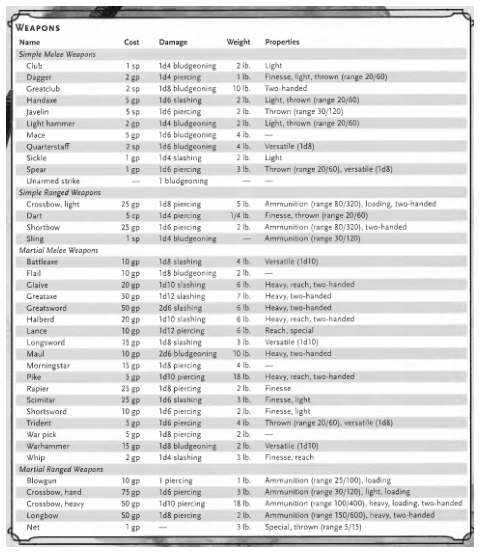
\includegraphics[width=0.57\textwidth]{Alarrak.png}
		\centering
	\end{figure}
	
	\subsection{Kompas}
	
	\begin{DndReadAloud}
		\sffamily
		Malá skleněná skříňka tvaru kulového vrchlíku. Kompas je obepnutý zdobnými pásky bronzového kovu abstraktních motivů a stejným materiálem je i zespodu vystužen. V~průzračné blískavé tekutině uvnitř plavou různobarevné střelky. Každá obyčejně ukazuje jinam.
	\end{DndReadAloud}
	
	Kompas neslouží k~rozpoznání světových stran. Pomáhá však s~cestováním svým vlastním způsobem. Bílá střelka kupříkladu vždy ukazuje k~meziostrovní bráně. Co dělají ostatní střelky vám nikdy nikdo nebyl schopný povědět. Někdy vám pomohou vyřešit hádanku brány, jindy vás nezavedou nikam.
	Kompas má také i pasivní schopnosti. Některé brány by bez jeho přítomnosti nebyly vůbec průstupné a u~mnoha dalších by bylo jejich aktivování komplikovaným procesem.
	
	\subsection{Nekonečný tlumok}
	
	\begin{DndReadAloud}
		\sffamily
		Jednoduchý béžovo-zelený batoh, který není tak obyčejný, jak se zdá. Každá z~jeho tří kapes je totiž zevnitř větší, a tak je pro Turisty stejně nepostradatelnou výbavou jako Kompas nebo Alarrak.
	\end{DndReadAloud}
	
	Tlumok má jednu hlavní a dvě boční kapsy; každá z~nich je extradimenzionální prostor. Boční kapsy unesou až 10kg materiálu o~maximálních rozměrech 1m$^3$ (2 krychlové stopy), hlavní až 40kg a 2,5m$^3$. Tlumok celý ale vždy váží jen 2,5kg.
	
	Ukládání věcí se řídí obvyklými pravidly zacházení s~předměty, vytahování vyžaduje akci -- chtěná věc se magicky objeví navrchu.
	
	Tlumok má omezení: pokud je přetížen nebo proražen či roztržen, roztrhne se celý a je nevratně zničen. Pokud se Tlumok zničí, jeho obsah se ztratí; jen vzácné artefakty se obvykle nakonec vyloupnou někde jinde. Pokud tlumok obrátíte naruby, všechen obsah se v~pořádku vysype. Jestliže do Tlumoku dáte dýchající bytost, bude mít kyslíku přibližně na deset minut; poté se začne dusit.
	
	Je-li vložen jeden tlumok do druhého, oba jsou instantně zničeny. Na místě, kde se toto stalo vznikne portál někam do prostoru, pravděpodobně (ale ne nutně) mimo jakýkoliv ostrov. Jakákoliv bytost v~okruhu 10 ft. od portálu je společně se všemi předměty uvnitř tlumoků vtažena dovnitř. Portál se následně okamžitě zavře a už nemůže být znovu otevřen.
	

	
	
	
	\part{Minulost}
	
	\chapter{Prydain}
	
	\DndDropCapLine{K}{}dysi dávno, před mnoha a mnoha lety, přišli na ostrov obři. Co bylo před nimi, nikdo neví; někdo říká, že ostrov byl obydlený a obři jednoduše vyhráli, někdo říká, že dávná civlizace dávno sama sebe vyhubila a obři přišli do divočiny, jiní zase, že zde žádná předchozí civilizace nebyla a prastaré ruiny jsou dílem obrů nebo lidí, co přišli po nich.
	
	Na tom by ještě tak nic nebylo; obři neuměli psát než svoje podivné a roztáhlé runy a vůbec toho po sobě moc nenechali, čemu by se dalo říkat \uv{civilizace}. Jenže jednoho dne se ostrov srazil s jiným, na kterém byli lidé, a tak se lidé dostali na ostrov a dali mu jméno Prydain.
	
	Říkali si \emph{Tuatha dé Danann}, a na nový ostrov Prydain je vedl král Nuada Airgetlám pojmenovaný tak pro svoji stříbrnou ruku. O tu svoji přišel v boji s obry, aby mu pak kovář Ogma a lékař Diancecht vyrobili novou ze stříbra. Mezi nimi byl také Lugh Llaw Gyffes, válečník s kouzelným kopím, který v druhé bitvě na poli Mag Tuired porazil království obrů, a od té doby byli obři jen v horách uprostřed Prydainu a na organizovaný odpor už se nezmohli. S lidmi také přišel na ostrov kouzelný kotlík krále Dagdy, jenž zůstal na původním ostrově, jemuž Tuatha dé Danann říkali Annwn. Poslední z nejslavnějších pokladů oněch lidí byl mocný meč Fragarach, jehož měl s sebou bratr Dagdy Lir, a později jej zdědil Lirův syn Manawydan.
	
	A tak začli lidé žít na Prydainu, a neměli toho mnoho, jen sami sebe a své schopnosti, které ovšem byly větší než dnes. Mezi Tuatha dé Danann vskutku bylo nezřídka výjimečných lidí a, snad to bylo oním věkem, snad lidmi, snad Prydainem, nezřídka kouzel. Tak i velký čaroděj Ogma měl tři učedníky a spolupracovníky. Enid, zběhlou ve vytváření kouzelných předmětů, Merlina, jenž teprv hledal svůj cíl, a Morrígan, jež zvládala předvídat osud jako nikdo jiný.
	
	Staletí ubíhala, a jak lidí přibývalo, ubývalo obrů i magie ve světě. I lidé se obrátili proti sobě a vedli spolu líté války a zakládali nová království a zase je bořili. Čas od času do dění vstoupil Merlin, tu aby poradil, tu aby kouzlem pomohl, aby pak znovu na desítky let zmizel.
	
	
	
	
	\chapter{Enid}
	\DndDropCapLine{E}{}nid pochází z ostrova Prydain. Z jejího vyprávění o ostrově by si zcestovalí Turisté, ostrovů a časů znalí, mohli myslet, že patří mezi velmi staré bytosti, ale opak budiž pravdou. Pyšní se teprve asi jednadvaceti zažitými léty. Po zjištění této skutečnosti následuje vždy od znalých Turistů otázka zásadní: \uv{Jak je to možné, co se stalo?}
	
	Enid většinou v reakci na tuto otázku pokrčí rameny, optá se tázajicího, zda je něco vůbec nemožné (jak pro Enid typické) a celkově toho o událostech vedoucích k jejímu skoku časem moc nenamluví. Možná za to může trauma způsobené vytržením ze známého prostřední, možná se s tím pojí skutečnost, kterou nikomu nechce vyzradit (třeba že vlastně neví), možná prostě a jednoduše ráda působí tajemně, či je to od každého trochu. Tázajicí se toho tedy od Enid moc nedozví. Jak to tedy bylo--nebylo? 
	
	Za devatero horami a devatero řekami byla jednou jedna malá chaloupka na kraji lesa, ve které se narodila malá holčička. Jak šel čas, malá holčička rostla a rostla, až se na nohy postavila. Nohy měla velmi neklidné, takže jakmile se na nich udržela, hnedka běžela objevovat svět. Nejprve se vydala s maminkou do vesnice, kde přičichla jako její otec kovadlině. Když trochu povyrostla, zamířila do lesa a každý den z něj něco přinesla, jednou uschlý list, podruhé prazvláštní larvu, potřetí to byl kus rudy -- a od té doby malá holčička nosila z lesa jen budoucí přátele kovadliny.
	Co na to říct, kovadlina se v krvi nezapře, říkala maminka malé holčičky vždy, když holčička z lesa přinesla kus rudy.
	
	Jak se holčička učila kovadlině, tak i její výtvory získávaly na kráse a funkčnosti. Jednoho dne se malá holčička, ze které se už stalo mladé děvče, rozhodla že jejím výtvorům něco chybí a vydala se hledat novou inspiraci hlouběji do lesa. Jak děvče šlo lesem, narazilo na jeskyni ve skále. Zvědavost mu nedala (ostatně jako vždy) a zamířilo vstříc hlubinám jeskyně. Co čert nechtěl, v jeskyni zrovna byl obr! Mladé děvče se velmi leklo, avšak po krátkém pozorování (a hlubokých úvahách nad smyslem života) si oddechla. Obr byl smrtelně raněn, ani už nedýchal. Zvědavost mu poručila a hned mělo ruce zabořené v obřích kapsách. Nejprve našlo jen starý kompas, pak se na něj ale štěstí usmálo, děvče našlo kov, co v životě nevidělo a hnedka zamířilo zpět domů ke kovadlině. Dalšího dne spatřil světlo světa medailonek z onoho kovu.
	
	Medailonek byl prazvláštní, mladé děvče se na něj nemohlo vynadívat, bylo na sebe neskutečně pyšné. Proto když se v rodinném kovářství objevil zákazník, který chtěl aby mu ukázala, co nejlepšího má. Ihned vytáhla medailonek. Když ho otevřela, zákazník spatřil malého kovového ptáčka pohybujícího křidélky a slyšel jeho zvučnou melodii. Stejně jako ona byl unešen, a tak se mladé děvče poháněné svou zvědavostí a touhou po nových znalostech stalo učněm onoho zákazníka. Zákazník, mistr Ogma, byl čaroděj a kovář. Krom našeho mladého děvčete měl ještě další dva učně: Morganu, ta byla jen o pár let starší než mladé děvče, a Merlina -- už se od svého mistra osamostatňoval.
	
	Mladé děvče trávilo ve společnosti mistra a jeho dalších učňů mnoho času, mistrovi pomáhala s kde čím. Jednou to byly očarované dveře se složitým mechanismem, jindy zase mistrovsky vyvedené pero bez náplně, či třeba svítící kovové květiny. Mistr Ogma toužil přijít na způsob, jak cestovat mezi ostrovy. Na to, proč po tom tak toužil, se ho jednou mladé děvče zeptalo, odpovědí byl jen zamyšelný pohled. Jednoho dne se mistr uprostřed práce náhle zastavil, rozesmál se a odběhl do své skryté pracovny, kterou mu děvče pomáhalo budovat. Vynořil se za dva dny, zrovna když si děvče hrálo se starým kompasem, co našlo před lety. Podíval se na děvče, usmál se, prohlásil: \uv{Tak jsem na to asi konečně snad přišel, zítra to vyzkoušíme.} a poté zmizel. Děvčeti zvědavost nedala, hned bylo v mistrově pracovně a hledělo na kovovou tyč na stole se zvláštní zástrčkou přibližně v půlce. Pak ji vzalo do ruky: \uv{To je na součástku, co dělám,} pomyslelo si a rozhodlo se, že to musí vyzkoušet a vydalo se ven z pracovny.	
	
	Ubohé zvědavé děvče prošlo branou a zatím znovu svůj pracovní stůl nespatřilo. Teď, jak se říká, zazvonil zvonec a pohádky je konec… nebo teprve začátek?
	
	\section*{Aby si čtenář udělal představu}
	Enid pochází z vesnice na kraji lesa, který obepíná Středohoří uprostřed ostrova. Středohoří tvoří pochopitelně hory, obývají ho obři. Lidé z Okraje lesa a obří vedou dlouhotrvající válku (nevedou neustále bitvy, spíš se sem tam servou o území). Mezi obry vládne hierarchie založená na vzrůstu, proto jsou menší obří často vyhošťováni a mnohdy nakonec pomáhají lidem se stavbou kde čeho oplátku za drobný peníz nebo něco k snědku. Enid je z Okraje, ale maminka jí od mala vtloukala, že obrům by se stavil jen blázen, pro má z vyšších lidí respekt a opravdu vyšších lidí se spíš bojí. I když, po setkání s malými obry ve městě poté, co šla do učení k mistrovi, už to není tak tragické...
	
	Když byla Enid v učení u mistra, tak vesnici jednou za dva týdny navštěvovala. Většinu času v rodné vesnici trávila buď v lese hledáním materiálů na kování, nebo kováním… Na vesnici žádné přátele neměla. Morgana Enid uvedla do společenského života, chodily společně do města se občas napít, občas zatancovat a stěžovat si na mistra jiným učňům čarodějů.
	
	Morgana seznámila Enid ve městě také s Ar. Enid učila Ar kovadlině a Ar Enid o okolní přírodě. Jinak si obě užívali společné útěky do lesa za dobrodružstvím. Jedna hledala kameny, druhá kytky. Aby se jim snáze dostávalo tak si pod dohledem mistra vytvořili létající koště (\emph{Broom of Flying}). Proto to byla jedna z prvních věcí, kterou si Enid po projití branou pořídila.
	
	Po projití branou si vyčítá svojí zvědavost a snaží se jí trochu krotit, ovšem jde jí to velmi špatně.  Mistr Ogma, sem tam nevrlý, je pro Enid velmi důležitá osoba. Zasvětil jí do tajů magie a dovedl jí tam kde je dnes, velmi k němu vzhlíží a neskutečně si cení jejich prvního společného výtvoru: konstrukt v podobě malého vrabce se srdcem z rubínu…Enid ho pojmenovala trefně, Vrabec.
	
	Jednoho dne by se ráda vrátila na Prydain, doufá, že jí to objasní, proč skočila časem a pomůže jí to vrátit se zpátky domů v čase. Rozpadání ostrovů tuto její naději ohrožuje. Enid prošla branou, když jí bylo devatenáct. Nemá problém sem tam porušit pravidla, když se dozví něco nového. Druidi jí připomínají Ar, takže jí připadají sympatičtí.
	
	
	
	
	
	
	
	\chapter{Cei}
	\begin{DndReadAloud}
		\sffamily
		\raggedright
		\uv{Bude míti jinou zvláštní vlastnost: je-li to můj syn, bude tvrdošíjný. Bude míti ještě jinou zvláštní vlastnost: když ponese břemeno, ať velké nebo malé, nebude ho nikdy viděti zpředu ani zezadu. Bude míti jinou zvláštní vlastnost: nikdo nevydrží oheň ani vodu tak dobře jako on.}\\
		\raggedleft Cynyr Ceinfarfog, \emph{Culhwch a Olwen}, \textsc{Mabinogi}
	\end{DndReadAloud}
	
	\DndDropCapLine{C}{}ei mab Cynyr se narodil na ostrově Prydain ve třetím věku od doby, co ho osídlili lidé, dvanáctý rok vlády emyra Arthura Pendragona. Ovšem svého otce, jenž mu do vínku nadělil proroctví jisté \emph{odolnosti}, jak vůči vůli ostatních, tak vůči vůli vnějších vlivů, nikdy nespatřil. Důvod mu matka nesdělila; možná pro jeho bezpečí, možná z úcty k Cynyrovi, možná z rozkazu emyra, možná ze strachu, možná prostě nevěděla. V každém případě Cei vyrůstal v divočině mimo Caerleon i Celliwig, mimo dosah dvora a dvorských mravů. Dětství a rané mládí strávil v Prydainských lesích na úpatí hor, v izolaci od civilizace jen se zvěří, lesem a zbytky dávných staveb obrů. \\
	
	Když mu bylo 12 let, jel okolo rytíř Řádu draka. Tehdy poprvé se Cei dozvěděl o existenci jiných lidí; nedlouho na to se odebral do Caerleonu, hlavního města. Usiloval zde o panošství pro některého ze slavných rytířů, ovšem pro svou tvrdohlavost a nepěstěné mravy příliš nepochodil a nakonec se stal kovářským učněm v Celliwigu.
	
	Jedenáct let strávil v žáru kovárny a naučil se kovat meče i zbroj jako málokdo, a jeho síla rostla a rostla. Až jednoho dne přišel do Celliwigu rytíř, oděný celý v zeleném a velký jako malý dům. V jedné ruce třímal velký a postaru zdobený meč, jaký by běžný smrtelník ztuha zvedl dvěma rukama, a všem přítomným rytířům přednesl výzvu. Kdokoliv že mu může oním mečem zasadit ránu, a za rok a den mu rytíř zasadí právě takovou. Odměnou bude odvážlivci meč. \\
	
	Žádný z přítomných rytířů výzvu nepřijal; mnoho z nich by nejspíš meč Zeleného rytíře vůbec nezvedlo. Až Cei, stále odhodlaný dokázat rytířům svoji hodnotu, zvedl jeho meč a jedinou ranou ho sťal. Ke zděšení všech však Zelený rytíř vzal do rukou svoji hlavu, zopakoval i druhou část výzvy, a odešel zpátky do hor. \uv{Do roka a do dne!}
	
	A tak byl Cei přijat mezi rytíře a ti obdivovali jeho odvahu. Ovšem Zeleného slova mu stále rezonovala v hlavě; setnout neobrněného obra je jedna věc, ale bojovat s nadpřirozenými silami je věc docela jiná, a obětovat život pro slávu a meč také. Zatvrzelost mu však nedovolovala výzvu vzdát a do hor za Zeleným rytířem nejet. Ukoval si tedy zbroj a odjel do Caerleonu, zjistit informace o Zeleném a poradit se s emyrem.
	
	\begin{figure}[t]
		\centering
	\noindent
	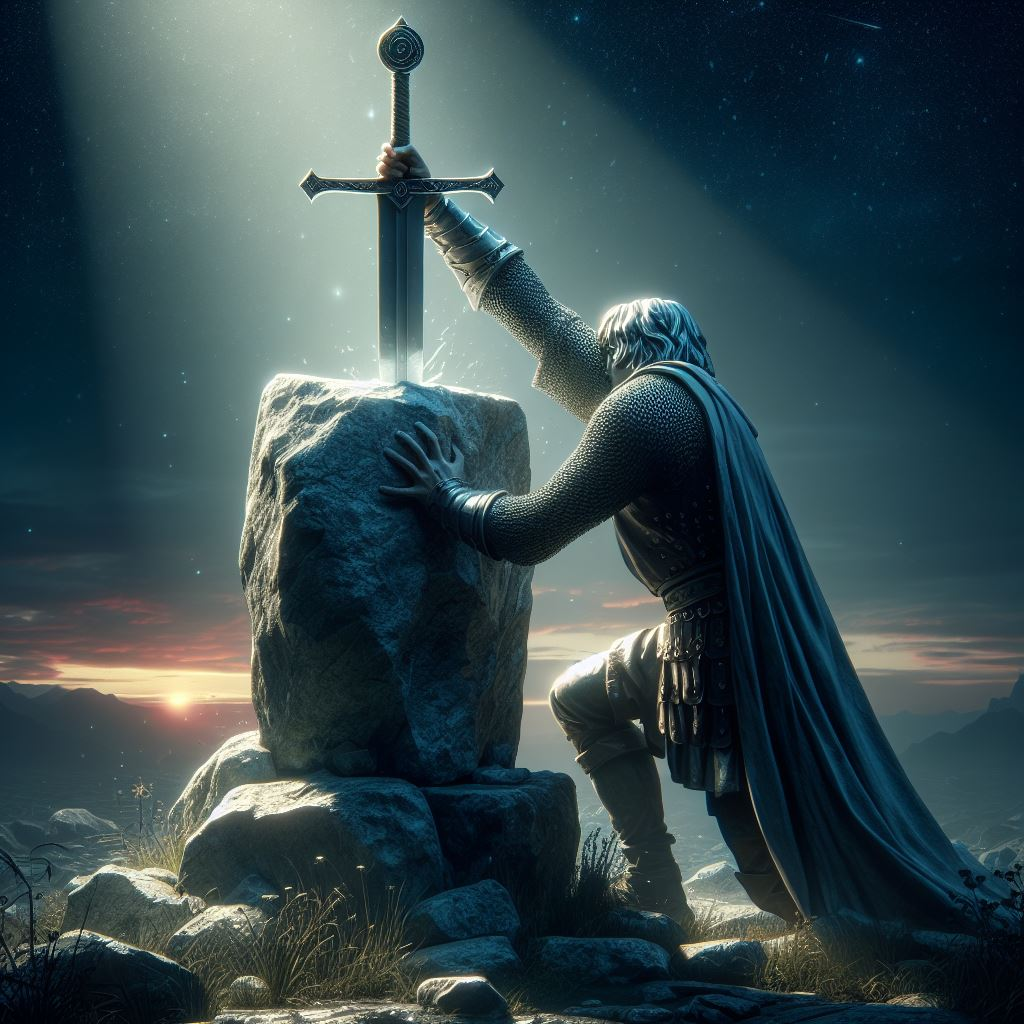
\includegraphics[width=\linewidth]{SwordInStone.jpg}
	\end{figure}
	
	V Caerleonu ale lidé už na podobné příběhy skoro zapomněli; při svých toulkách po lese, kde vyrůstal, se s tím co zbylo po obrech setkal více, než většina obyvatel Caerleonu dohromady. V polovině zadaného intervalu posedl Ceie zvláštní vztek, zvláštní zuřivost, jenže v Caerleonském hradě nebylo, jak ji vybít nebo proti komu namířit. A v takovém stavu se Ceiovi zdál následující sen. V něm byl hrad jako v Caerleonu, jenže se rozpadal; král jako Arthur, ale starý a nemohoucí. V jeho síni viselo na čestném místě zvláštní kopí -- příliš velké, aby jím běžný člověk dokázal hodit, ale velce krásně vykované a zjevně použité; vedlejší hák na trofejní meč byl prázdný. Před trůnem stál jiný podivný předmět: buď neobvykle široký \uv{kalich} nebo kratér, nebo kotlík s jednonohým podstavcem. Cei přistoupil a podíval se do toho předmětu a spatřil obraz překrásné dívky ve starobylém šatu. Ovšem obraz se za chvíli rozplynul do podoby postavy v černém, jak provádí nějaký rituál, a chvíli na to se ozvala strašná rána a Cei vzhlédl. Kopí na stěně bylo zlomené a králi se začaly objevovat na těle rány, když v tom sen skončil. Cei se probudil ve své komnatě, celkem zdemolované, a všude po hradě byl povyk a shon. Ne však kvůli Ceiovi; po chvíli ptaní se dozvěděl, že z Prydainu se odlomil kus velký jako průměrná vesnice i s přilehlými poli, naštěstí neobývaný.
	
	Zvláštní vize motivovala Ceie, aby více prozkoumával Caerleonský hrad. A vskutku, nakonec našel v zapadlém sklepení kotlík ze snu -- to už se blížil zadaný termín -- a v něm obraz jeho samého se zelenou páskou okolo krku. Cei po ní sáhnul -- a obraz zmizel a hedvábná zelená páska se mu objevila v ruce.
	
	Ještě než nadešel onen den, vypravil se Cei do hor vyhledat Zeleného rytíře. Našel ho, s hlavou nasazenou, ve stavu jakéhosi spánku nebo hibernace, v jedné z prastarých budov v samém středu Prydainu. Měla skoro kruhový půdorys, kamenné obvodové zdi, hliněný strop porostlý travou a jediný mohutný sloup přímo uprostřed; uvnitř byla prakticky tma. Cei si tedy nasadil zelenou pásku a čekal.
	
	O půlnoci, velice světlé, neboť byl úplněk, přesně rok a den od prvního setkání, se Zelený rytíř probudil, vzal do rukou svůj meč, viděl Ceie stojícího klidně před sebou -- \emph{a máchl}.
	
	\vspace{1\baselineskip}
	
	\noindent
	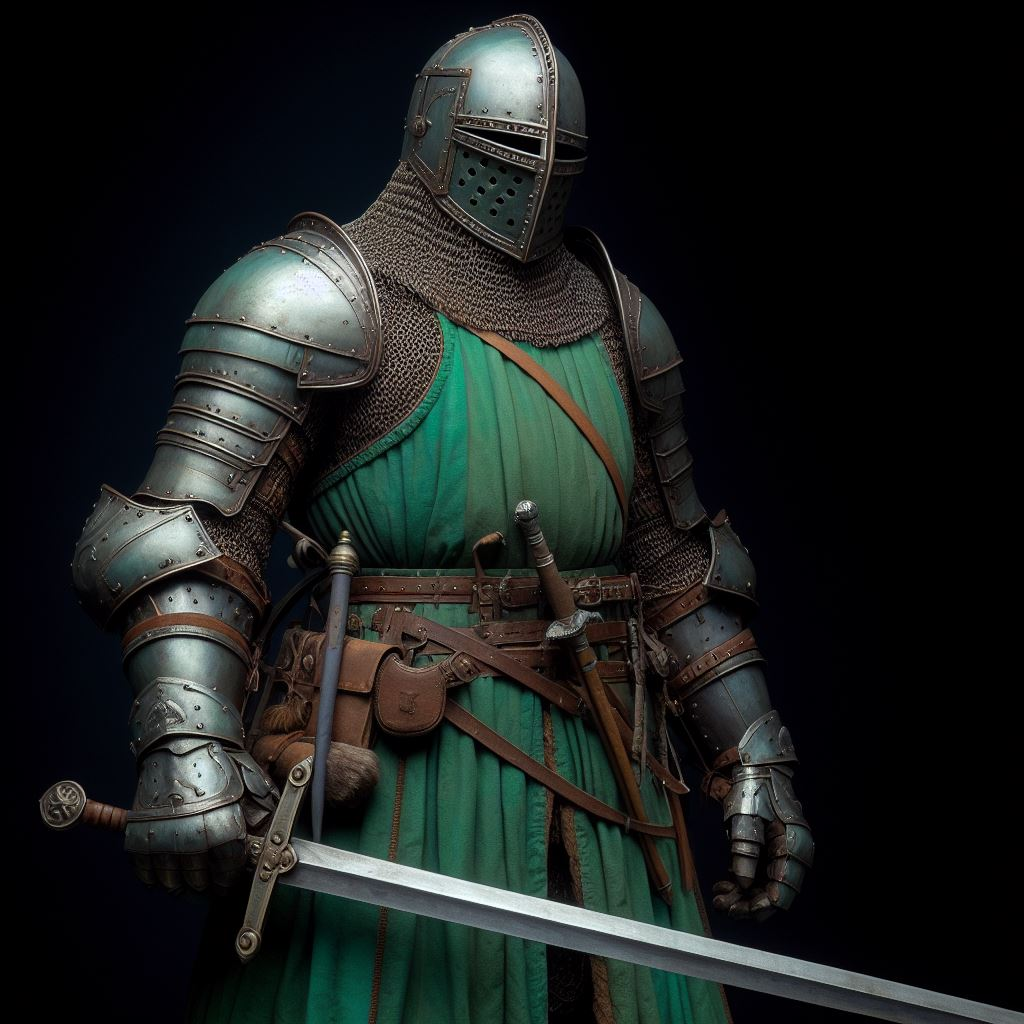
\includegraphics[width=\linewidth]{GreenKnightPlain.jpg}
	
	\vspace{2\baselineskip}
	
	\begin{DndReadAloud}
		\sffamily
		\raggedright
		Cei měl zvláštní vlastnost: devět dní a devět nocí vydržel beze spánku. Ránu Ceiova meče nemohl lékař vyléčiti. Cei byl znamenitý člověk; když se mu zlíbilo, byl tak vysoký jako nejvyšší strom v lese. Měl jinou zvláštní vlastnost: i za největšího deště to, co držel v ruce, bylo suché na dlaň nad jeho rukou a dlaň pod ní, tak veliký byl jeho žár. A když jeho druhům bylo nejvíce zima, zapaloval jim oheň svým vlastním žárem.\\
		\raggedleft \emph{Culhwch a Olwen}, \textsc{Mabinogi}
	\end{DndReadAloud}
	
	Ceiovi se zdálo o panně z vize v kotlíku. Když se Cei probral, byla opět tma. Všechno ho bolelo a chvíli trvalo, než se zvedl zpátky na nohy. Zapálil si louči a rozhlédl se okolo sebe.
	
	Kus od něj ležel Zelený rytíř, přibodnutý mečem k zemi, už mírně v rozkladu. Cei šel a zabral za meč -- přeci jen, měla to být odměna, a Zelený rytíř už ho zjevně nevyužije. Zabral poprvé, meč nepovolil. Zabral podruhé a meč se mírně zachvěl. Zabral potřetí -- a meč povolil, i s kusem skály... Ale měla to být jeho odměna, a nějaká skála ho jen tak nezastaví. Poté si Cei vzpomněl, co se dělo předtím, a sáhl si na krk. Zelená páska tam stále byla, ale když se podíval na svoje prsty, byl na nich tenký proužek krve...
	
	\DndDropCapLine{Z}{}pátky v Caerleonu mezitím uběhl celý rok a nikdo nepředpokládal, že se Cei ještě vrátí. Tomu ale stále ležela na srdci záhadná kráska, a tak znovu vyhledal onen kotlík. Tentokrát v něm ovšem nebyl obraz krásné dívky, ale hůl z neznámého materiálu a jakási skříňka se sklíčkem zasazeným do zdobného bronzového kovu s jednou bílou a pár dalšími střelkami a obyčejně vypadající brašna. Zklamán, Cei si ony předměty vzal, a šel dál. Jenže když procházel podivně kruhovou branou, která stála na konci místnosti s kotlíkem, najednou zjistil, že je někde úplně jinde...
	
	
	\part{Přítomnost}
	\section{Sezení 1}
	Po průchodu branou jsme se objevili na ostrově, jenž je, aspoň můžu-li tvrdit, jedna velká hospoda. Což není vůbec od věci, ostatně soudím, že tak dobře už jsem se dlouho nenajedl. Přivítal nás pan \uv{Hospodský}, samozřejmě jídlem a pitím, jak se sluší. Zjevně máme být něco jako \uv{družina} mezi \uv{Turisty}, ať už to znamená cokoliv.
	
	Než jsme dorazili, konverzace se pravděpodobně točila kolem předchozí družiny Turistů, kteří se vrátili z nějaké údajně 
	
	\part{Seznam NPC}
	\section{1. ostrov}
	\subsection{Hospodský}
	\bi
		\item Friendly
		\item Tajemné NPC
		\item Hospodský ostrov, jedna velká hospoda
		\item centrála Turistů?
		\item Přiměl naši družinu stát se družinou, přísahat
		\item Poslal nás na první quest, zjistit, co se stalo s Vladovou družinou
	\ei
	\subsection{Hubertus}
	
	
	
\end{document}